%run latex file, dvips file, ps2eps file

\documentclass{article}

% amsmath package, useful for mathematical formulas
\usepackage{amsmath}
% amssymb package, useful for mathematical symbols
\usepackage{amssymb}

% graphicx package, useful for including eps and pdf graphics
% include graphics with the command \includegraphics
\usepackage{graphicx}

% cite package, to clean up citations in the main text. Do not remove.
\usepackage{cite}

\usepackage{color} 

\usepackage{tikz} \usetikzlibrary{automata}
\usetikzlibrary{arrows,snakes,backgrounds}

\begin{document}
\thispagestyle{empty}

\begin{minipage}{0.3\linewidth}
  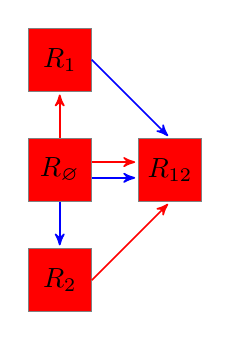
\begin{tikzpicture}[node distance=1.4cm, inner sep=0pt, minimum size=8mm]
    \tikzstyle{seb}=[rectangle, fill=red, draw=gray, text=black]
    \tikzstyle{I1}=[->, draw=red, shorten >=1pt, >=stealth',semithick]
    \tikzstyle{I2}=[->,draw=blue, shorten >=1pt, >=stealth',semithick]

    \node[seb] (R0) {$R_\varnothing$};
    \node[seb] (R1) [above of=R0] {$R_1$};
    \node[seb] (R2) [below of=R0] {$R_2$};
    \node[seb] (R12) [right of=R0] {$R_{12}$};

    \draw[I1] (R0) to (R1);
    \draw[I2] (R0) to (R2);
    \draw[I2] (R1.east) to (R12.north);
    \draw[I1] (R2.east) to (R12.south);
    \draw[I1] ([yshift=+1mm] R0.east) to ([yshift=+1mm] R12.west);
    \draw[I2] ([yshift=-1mm] R0.east) to ([yshift=-1mm] R12.west);
\end{tikzpicture}
\end{minipage}
%%%%%%%%%%%%%%%%%%%%%%%%%%%%%%%%%%%%%%%%%%%%%%%%%%%%%%%%%%%%%%%%%%%%%%%%%
% SBRI
%%%%%%%%%%%%%%%%%%%%%%%%%%%%%%%%%%%%%%%%%%%%%%%%%%%%%%%%%%%%%%%%%%%%%%%%%
\begin{minipage}{0.3\linewidth}
  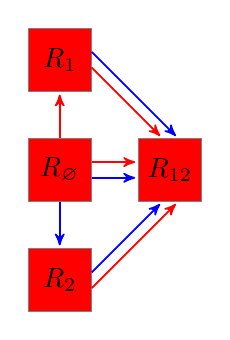
\begin{tikzpicture}[node distance=1.4cm, inner sep=0pt, minimum size=8mm]
    \tikzstyle{seb}=[rectangle, fill=red, draw=gray, text=black]
    \tikzstyle{I1}=[->, draw=red, shorten >=1pt, >=stealth',semithick]
    \tikzstyle{I2}=[->,draw=blue, shorten >=1pt, >=stealth',semithick]

    \node[seb] (R0) {$R_\varnothing$};
    \node[seb] (R1) [above of=R0] {$R_1$};
    \node[seb] (R2) [below of=R0] {$R_2$};
    \node[seb] (R12) [right of=R0] {$R_{12}$};

    \draw[I1] (R0) to (R1);
    \draw[I2] (R0) to (R2);
    \draw[I2] ([yshift=+1mm] R1.east) to ([xshift=+1mm] R12.north);
    \draw[I1] ([yshift=-1mm] R2.east) to ([xshift=+1mm] R12.south);
    \draw[I1] ([yshift=-1mm] R1.east) to ([xshift=-1mm] R12.north);
    \draw[I2] ([yshift=+1mm] R2.east) to ([xshift=-1mm] R12.south);

    \draw[I1] ([yshift=+1mm] R0.east) to ([yshift=+1mm] R12.west);
    \draw[I2] ([yshift=-1mm] R0.east) to ([yshift=-1mm] R12.west);
\end{tikzpicture}
\end{minipage}
%%%%%%%%%%%%%%%%%%%%%%%%%%%%%%%%%%%%%%%%%%%%%%%%%%%%%%%%%%%%%%%%%%%%%%%%%
% HB
%%%%%%%%%%%%%%%%%%%%%%%%%%%%%%%%%%%%%%%%%%%%%%%%%%%%%%%%%%%%%%%%%%%%%%%%%
\begin{minipage}{0.3\linewidth}
  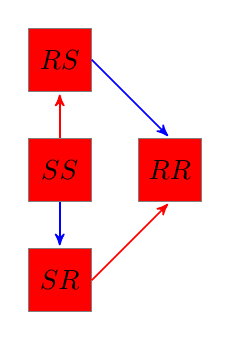
\begin{tikzpicture}[node distance=1.4cm, inner sep=0pt, minimum size=8mm]
    \tikzstyle{seb}=[rectangle, fill=red, draw=gray, text=black]
    \tikzstyle{I1}=[->, draw=red, shorten >=1pt, >=stealth',semithick]
    \tikzstyle{I2}=[->,draw=blue, shorten >=1pt, >=stealth',semithick]

    \node[seb] (R0) {$SS$};
    \node[seb] (R1) [above of=R0] {$RS$};
    \node[seb] (R2) [below of=R0] {$SR$};
    \node[seb] (R12) [right of=R0] {$RR$};

    \draw[I1] (R0) to (R1);
    \draw[I2] (R0) to (R2);
    \draw[I2] (R1.east) to (R12.north);
    \draw[I1] (R2.east) to (R12.south);
\end{tikzpicture}
\end{minipage}

\end{document}
